% Copyright (C) 2010,2011,2012 The ESPResSo project
% Copyright (C) 2002,2003,2004,2005,2006,2007,2008,2009,2010 
%   Max-Planck-Institute for Polymer Research, Theory Group
%  
% This file is part of ESPResSo.
%   
% ESPResSo is free software: you can redistribute it and/or modify it
% under the terms of the GNU General Public License as published by the
% Free Software Foundation, either version 3 of the License, or (at your
% option) any later version.
%  
% ESPResSo is distributed in the hope that it will be useful, but
% WITHOUT ANY WARRANTY; without even the implied warranty of
% MERCHANTABILITY or FITNESS FOR A PARTICULAR PURPOSE.  See the GNU
% General Public License for more details.
%  
% You should have received a copy of the GNU General Public License
% along with this program.  If not, see <http://www.gnu.org/licenses/>.
%
%%%%%%%%%%%%%%%%%%%%%%%%%%%%%%%%%%%%%%%%%%%%%%%%%%%%%%%%%%%%%%%%% 
% From the brainstorming:
%
% Preknowledge:
% 
% Basic MD(simple integrator,langevin thermostat, ---basic tcl
% basic potentials, basis tutorial 1
% 
% Basis Tutorial: written in Latex
% 
% <<every line of script code should be explained>>
% 
% 1) tcl basic setting up a system
% MD, soft sphere and Lennard-Jones Fluid (argon system), 
% Units
% 
% online visualization (pdb output)
% rdf, pressure,energy,
% 
% online analysis function
% savin, readin, writeout, offline analysis, statistics
% 
% Structure:
% Part1:
% 1) Prerequisites (what you should know beforehand: basic tcl knowledge,
% Here you can find more info: Allen, Tildesley: Frenkel Smit,
% Rappaport, Tcl tutorial,
% 
% 2) Physics of the systems (argon, soft sphere system)
% 
% 3) Algorithms (verlocity verlet, Langevin, Potentials, LJ)
% 3b) about units
% 
% Part2 
% 1) simulation script in all detail, line by line
% Initialize
% Visualize
% Simulate (with online analysis, saves for later off-line analysis,
% (Savelize (save our lives ))
% 
% 2) a new script for later
% analysis, and other helper ideas
% 
% Things to remember and take care of:
% Use the same names for variables
% 
% ====================================================================
% General Tutorial: (the next tutorials: pe_solution, cell model of one
% charged colloid, LB, ferrofluid)
% 
\documentclass[
paper=a4,                       % paper size
fontsize=11pt,                  % font size
twoside,                        % two sided
footsepline,                    % add a line to separate the footer
headsepline,                    % add a line to separate the header
headinclude=false,              % header does not belong to the text
footinclude=false,              % footer does not belong to the text
pagesize,                       % set the pagesize in a DVI document
]{scrartcl}

% Copyright (C) 2010,2011,2012,2013,2014,2015,2016 The ESPResSo project
% Copyright (C) 2002,2003,2004,2005,2006,2007,2008,2009,2010
%  Max-Planck-Institute for Polymer Research, Theory Group
%  
% This file is part of ESPResSo.
%   
% ESPResSo is free software: you can redistribute it and/or modify it
% under the terms of the GNU General Public License as published by the
% Free Software Foundation, either version 3 of the License, or (at your
% option) any later version.
%  
% ESPResSo is distributed in the hope that it will be useful, but
% WITHOUT ANY WARRANTY; without even the implied warranty of
% MERCHANTABILITY or FITNESS FOR A PARTICULAR PURPOSE.  See the GNU
% General Public License for more details.
%  
% You should have received a copy of the GNU General Public License
% along with this program.  If not, see <http://www.gnu.org/licenses/>.
%
\usepackage[draft]{varioref}    % defines \vref
\usepackage{hyperref}           % automatically creates links when
                                % using pdflatex, defines \url
\usepackage{ifpdf}              % defines \ifpdf
\usepackage{graphicx}           % handles graphics
\usepackage{color}              % use colors

\usepackage{amsmath}

\usepackage{verbatim}           % required for \verbatim and \endverbatim
\usepackage{fancyvrb}
\usepackage{calc}               % compute length
\usepackage{ifthen}             % provide ifthen
\usepackage{xspace}
\usepackage{units}
\usepackage[numbers]{natbib}

% For building the distribution docs, disable todo boxes.
%\usepackage[disable]{todonotes}
\usepackage{todonotes}

\newcommand{\es}{\mbox{\textsf{ESPResSo}}\xspace}
\newcommand{\ie}{\textit{i.e.}\xspace}
\newcommand{\eg}{\textit{e.g.}\xspace}
\newcommand{\etal}{\textit{et al.}\xspace}

\newcommand{\codebox}[1]%
{\texttt{#1}}

\DefineVerbatimEnvironment{code}{Verbatim}%
{commandchars=\\\{\}}
\makeatletter
\newenvironment{tclcode}
{%
  \addtolength{\linewidth}{-2em}% set the line length
  \@minipagetrue%%%DPC%%%
  \@tempswatrue%%%DPC%%%
  \hsize=\linewidth%
  \setbox0=\vbox\bgroup\verbatim
}{\endverbatim
  \unskip\setbox0=\lastbox%%%DPC%%%
  \egroup
  \par%
  \noindent\hspace{1em}%
  \codebox{\box0}%
  \par\noindent%
}
\makeatother

% \newcommand{\todo}[1]{
%   \marginpar{%
%     \setlength{\fboxrule}{1pt}
%     \fcolorbox{red}{yellow}{%
%       \parbox{\marginparwidth-2\fboxrule-2\fboxsep}{%
%         \bf\raggedright\scriptsize #1%
%       }%
%     }%
%   }%
% }

\makeatletter
\renewcommand{\minisec}[1]{\@afterindentfalse \vskip 1.5ex
  {\parindent \z@
    \raggedsection\normalfont\sffamily\itshape\nobreak#1\par\nobreak}%
  \@afterheading}
\makeatother

\newcommand{\esptitlehead}{
  \titlehead{
    \begin{center}
      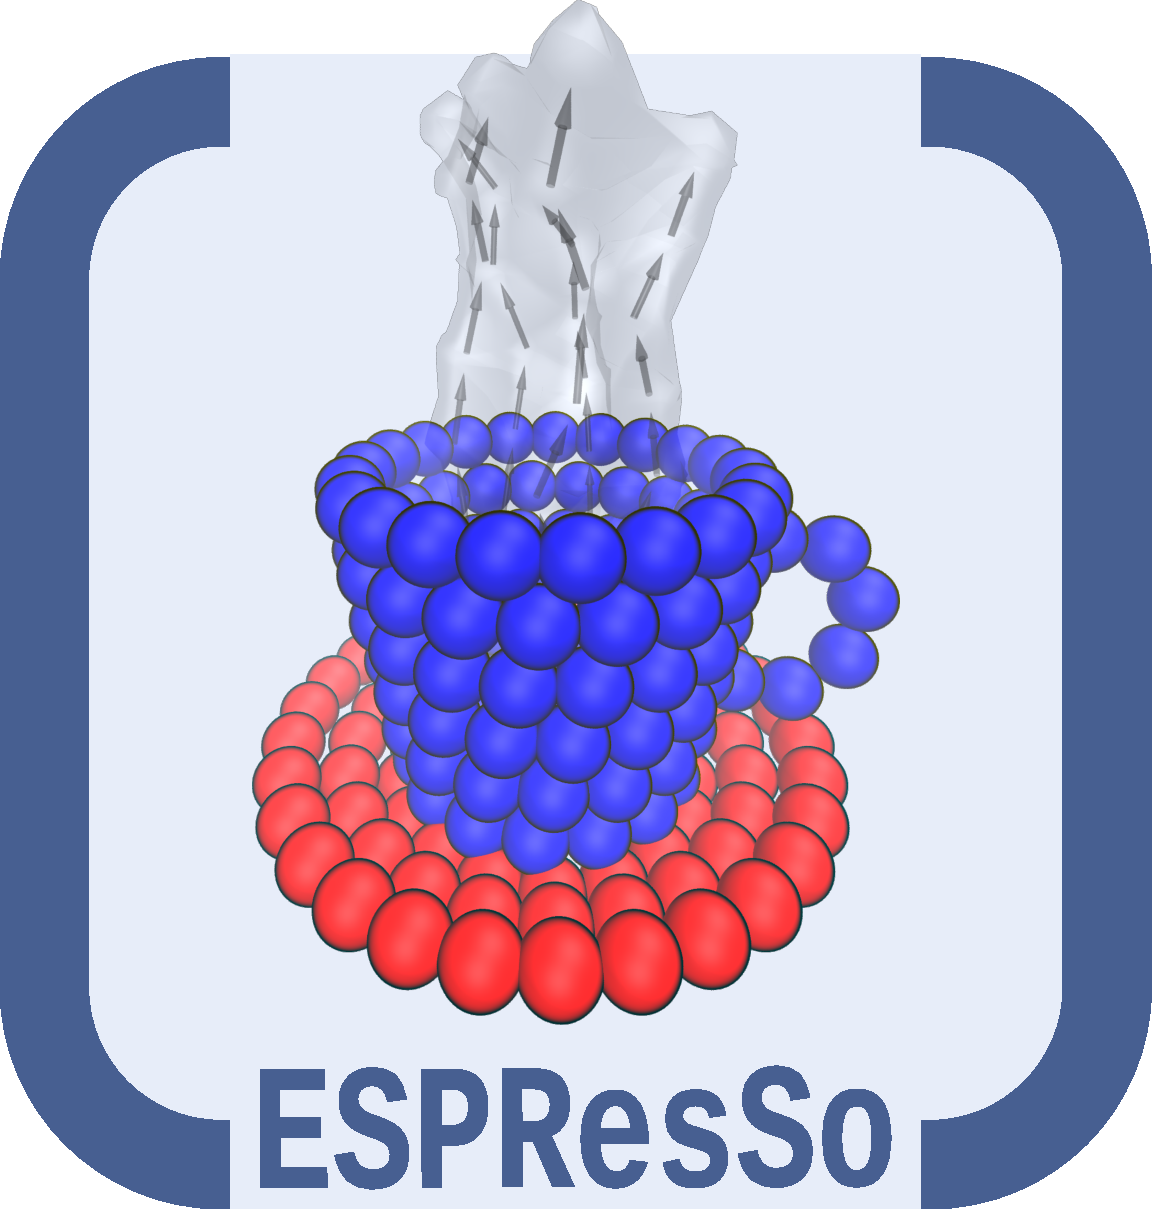
\includegraphics[width=5cm]{logo/logo.pdf}
    \end{center}
  }
}


%% Grafikpakete
\usepackage{graphicx}%
\usepackage{verbatim}

% How to diplay ESPResSo commands in flowing text. Larger code segments
% should be put inside boxes.
\newcommand{\EScmd}[1]{\texttt{\textbf{#1}}}

% The code block
%\newcommand{\EScode}[1]{ \parbox{0.95\textwidth}{\texttt{#1}}}
\usepackage{listings} 
\lstset{numbers=left, numberstyle=\tiny, numbersep=5pt, showspaces=false, showstringspaces=false,postbreak=\space, breakindent=5pt, breaklines}
\lstset{language=tcl, keywordstyle=\color{blue}\bfseries ,emphstyle=\color{green}, commentstyle=\color{red}\itshape }
\lstset{keywordsprefix=setmd}
\lstset{keywords=[6]{thermostat,part,inter,integrate,rescale_velocities,code_info,save_sim,writepdb,analyze,uwerr}}

\newtheorem{task}{Task}

\begin{document}

\esptitlehead

\title{Tutorial 1: The Lennard-Jones Liquid%
\ifdefined\esversion%
\thanks{For \es \esversion}%
\fi%
}
\subtitle{\es Basics}
\author{H.-J. Limbach \and M. S\"uzen \and K. Grass \and M. Sega \and A. Arnold \and N. Gribova \and J. de Graaf}
\maketitle
\tableofcontents

\section{Introduction}

Welcome to the basic \es{} tutorial! In this tutorial, you will learn, how to use the \es{} package for your research. We will cover the basics of \es, i.e.~how to set up and modify a physical system, how to run a simulation, and how to save, load, and analyze the data.

The more advanced features and algorithms available in the \es{} package are described in the other tutorials, which will be developed further and expanded upon in the future.

\section{Background}

Today's research on Soft Condensed Matter necessitates having a flexible, extensible, reliable and efficient (parallel) molecular simulation package. For this reason \es{} (Extensible Simulation Package for Research on Soft matter) \cite{esp_url} has been developed at the Max Planck Institute for Polymer Research, Mainz by the Group of Prof. Dr. Christian Holm \cite{limbach2006ees}. The Espresso package is probably the most flexible and extensible simulation package that is currently available. It was specially developed for coarse-grained molecular dynamics (MD) simulations of polyelectrolytes, but it is not necessarily limited to such systems. \es{} can, for example, even be used to simulate granular media. The quality and usefulness of \es{} have been recognized throughout the field, resulting in a nomination for the Heinz-Billing-Preis for Scientific Computing in 2003 \cite{arnold2003ees}.

\section{Tutorial Outline}

In this short tutorial, you will be introduced to the \es{} package as gently as possible, with only a minimal set of skills as a prerequisite. We will guide you through the initial steps of working with \es{} and help you to examine a simple physical system, namely a Lennard-Jones liquid.

After a brief introduction to \es{} in Section~\ref{sec:espresso}, we provide you with a short tutorial on the Tcl programming language which is used to control \es{} simulations in Section~\ref{sec:tcl}. In Section~\ref{sec:ljliquid}, we will introduce you to the system of interest and familiarize you with the necessary background knowledge. Please note, however, that it is beyond the scope of this tutorial to give a complete overview of the the area. We will therefore provide a few references in which you can find more detailed information regarding MD. Finally, in Section~\ref{sec:ana} we use \es{} to analyze the data we obtained from our simulation and we study the physical properties of the system. 


\section{\label{sec:espresso}First steps}

What is \es{}? It is not coffee, indeed. It is an extensible, efficient Molecular Dynamics package, that from its inception was designed to be a particularly powerful platform for the simulation of charged systems. Over the years it has grown to encompass many more systems. In depth information on the available packages can be found on the \es{} website~\cite{esp_url}, in the User Guide\footnote{Available on the \es{} website~\cite{esp_url} and in every release under the \texttt{doc/ug} folder.} and the (recent) papers~\cite{arnold2003ees,limbach2006ees,Roehm2012}.

From the user's point of view, \es{} is driven by Tcl(/TK)\footnote{Tool command language, pronounced `tee-cee-el' or `tickle'.}~\cite{tcl_url}. That is, the user can interact with the package core by typing Tcl commands into the command line interface (CLI) or via scripts written in the Tcl scripting language\footnote{In short, a \emph{scripting language} allows the user to write instructions that are carried out by an interpreter without prior compiling. This enables the user to use \es{} for vastly different applications without the need of different specialized executable files.}. Currently, all versions of \es{} have CLI enabled, but \emph{user be warned!} Tcl commands input into the CLI directly may give unexpected and undesirable results. Moreover, the CLI is known to have serious functionality problems for non-POSIX systems. It is \emph{highly} recommended that Espresso is driven using scripts only. 

In a given \es{} script, some commands are interpreted by the scripting language (Tcl), while others by the core \es{} program written in C. However, all \es{} commands and directives in the script are transparent to the user, regardless of its implementation either on the C- or Tcl-level.

\emph{Note: This tutorial assumes that you already have a working \es{} installation on your system. If this is not the case, please go to \texttt{http://www.espressomd.org/} for information on how to obtain and install \es{}.}

\vspace{1cm}
\framebox{
\begin{minipage}{0.95\textwidth} 
\begin{task} \label{task:start}
To start \es{}, simply type \texttt{Espresso} (or \texttt{./Espresso}) in the command line shell. This will open the Command Line Interface (CLI) of \es{}. Upon issuing the \es{} command \lstinline|code_info| you can see the options that are included in your \es{} binary\footnote{\es{} provides many different features, some which are mutually exclusive. This is why not all features are activated by default, but instead have to be explicitly requested at compile time of the executable. Please consult the User Guide for details on this.}. N.B. This option may not be default in \es{} versions that follow the 3.1.1 release. If you want to experiment with the Tcl part of this tutorial in a version of \es{} that does not have the CLI default, you can also use the \texttt{tclsh} program, which can be installed on any POSIX OS and functions as a simple Tcl command line interpreter.
\end{task}
\end{minipage}}
\vspace{1cm}

\begin{figure}[htp]
\begin{center}
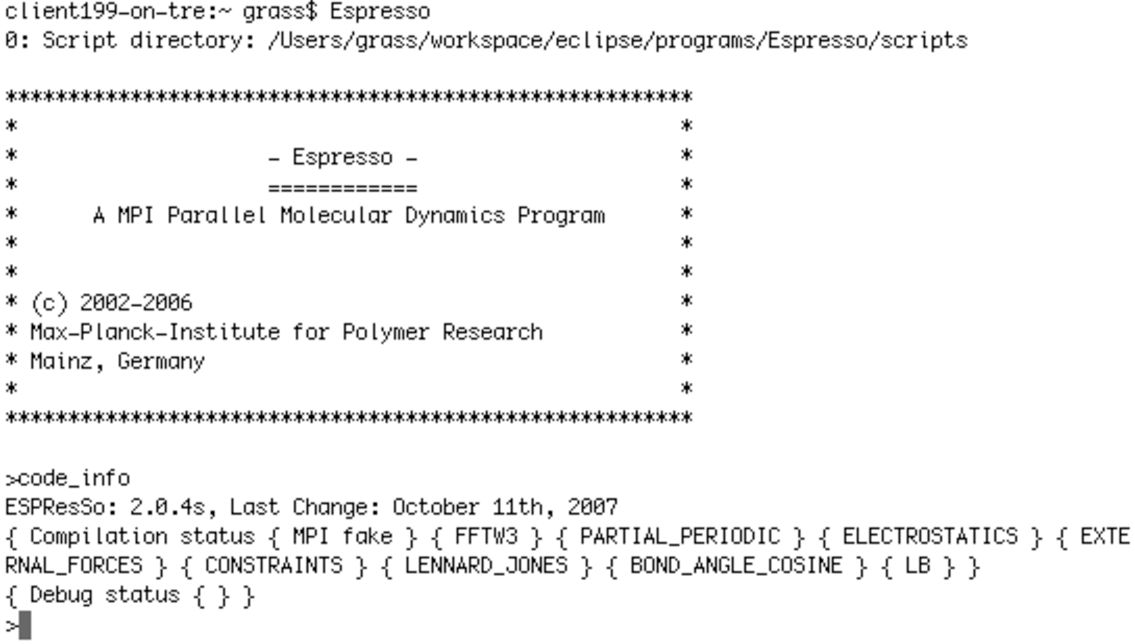
\includegraphics[width=0.75\textwidth]{figures/espresso-output.pdf}
\caption{\label{fig:espresso_output} Example output of the \es{} Command Line Interface (CLI) upon issuing the \lstinline|code_info| command.}
\end{center}
\end{figure}

\vspace{1cm}
\framebox{
\begin{minipage}{0.95\textwidth} 
\begin{task}
Figure~\ref{fig:espresso_output} shows the terminal output you should have obtained. What kind of output are you receiving from  \lstinline|code_info| command?
\end{task}
\end{minipage}}
\vspace{1cm}

On the screen shot in Fig.~\ref{fig:espresso_output} you can see several in-compiled features, e.g.~the fast Fourier transformation (FFTW), the Lennard Jones and electrostatic potential, and the parallel computing feature (MPI\_CORE). All features are explained in the \es{} User Guide.

\section{Short Tcl Tutorial}\label{sec:tcl}

Tcl (Tool Command Language) is a very powerful, yet easy to learn programming language.\footnote{It is dynamically interpreted, which means that commands are read, interpreted, and executed by the computer one command line at a time. N.B. As of version 3.1.1 attempts are made to eventually replace the Tcl interface with a Python based one. The current \es{}++ version (basically a C++ version of \es{}, with slightly different feature) already employs a Python interface.} Aside from any valid Tcl code, the user can provide \es{} with any valid \es{} command using the CLI.\footnote{Again, this option may not be default in \es{} versions that follow the 3.1.1 release.} In the following, we give a basic Tcl tutorial, which is based on Ref.~\cite{tcl_tut_url}, that can be made using the Espresso CLI. Type \texttt{Espresso} to obtain the \es{} command line interface, also see Task~\ref{task:start}. Once in the CLI, you can familiarize yourself with the basics of Tcl. 
   
\subsection{Assignments and evaluation}

A simple text output, or a print statement can be carried out with \lstinline|puts| \footnote{Valid Tcl / \es{} commands are bold and blue, all following code can be direct used with \es{}.}
      
{\vspace{0,2cm}\small
\begin{lstlisting}[numbers=none]
puts "Hello Espresso \n"
puts "\t tab \t another tab,\n and a new line"
puts "This is line 1"; puts "this is line 2"
puts "1.2";	# this is a comment
\end{lstlisting}\vspace{0,2cm}
}

C-like backslash sequences can be used along \lstinline|put|. For example, \texttt{\textbackslash{}t} puts a tab, \texttt{\textbackslash{}r} puts a line return and \texttt{\textbackslash{}n} puts a carriage return. Comments are placed using a hash (\#) sign. It should be noted that regular Tcl commands may be followed by a semicolon `;' symbol to close the line. N.B. This is required if you end-comment a statement or if you want to put multiple statements on one line. 

\noindent In order to declare a variable and/or assign a value to it, you use the assignment command, called \lstinline|set|.

{\small\vspace{0,2cm}
\begin{lstlisting}[numbers=none]
set X "This is a string"
set Y 1.24
puts $X
puts $Y
\end{lstlisting}\vspace{0,2cm}
} 

\noindent When assigning a value to a variable, the variable is accessed simply by its variable name (as in the first line, \texttt{X}). When a value is accessed, the variable name is preceded by a dollar sign (as in the third line, \texttt{\$X}).

To evaluate the result of mathematical expressions you can use the \lstinline|expr| command. Note, that the entire statement is enclosed in square brackets. 

{\small\vspace{0,2cm}
\begin{lstlisting}[numbers=none]
set X 60
set Y 30
set Z [expr $X+$Y]
puts "X=$X and Y=$Y and X+Y=$Z"
\end{lstlisting}\vspace{0,2cm}
}

\noindent Most C-like operators and math functions are valid Tcl syntax.

{\small\vspace{0,2cm}
\begin{lstlisting}[numbers=none]
set X 2
set cosX [expr cos($X)]
puts "cos($X) = $cosX"
\end{lstlisting}\vspace{0,2cm}
}

\subsection{Comparisons and looping}

The syntax for numeric comparison using the \lstinline|if| command is as follows 

{\small\vspace{0,2cm}
\begin{lstlisting}[numbers=none]
set x 5
if {$x == 5} {puts "$x is 5"} else {puts "$x is not 5"}
\end{lstlisting}\vspace{0,2cm}
} 
      
\noindent You may also write this in different lines by using backslashes. As in many shell scripting languages, including Tcl, the  backslash is used for line continuation. You must use this to achieve line continuation in the \es{} CLI, but it is not necessary when running a loaded script. \emph{There is one exception:} even in a script, Tcl expects all parameters of a function, including flow control commands such as \texttt{if} or \texttt{while}, to be on the same line. Therefore, you may need continuation backslashes even in a script. However, a block with in curled braces, which is the most common in Tcl, does not require backslashes for continuation inside. To clarify this difference we give two \emph{script} examples. In a script, the above code might look like this: 

{\small\vspace{0,2cm}
\begin{lstlisting}[numbers=none]
set x 5
if {$x == 5} {
  puts "$x is 5"
} else {
  puts "$x is not 5"
}
\end{lstlisting}\vspace{0,2cm}
}

\noindent However, you still need the backslashes in this style:

{\small\vspace{0,2cm}
\begin{lstlisting}[numbers=none]
set x 5
if {$x == 5} \
  { puts "$x is 5" } \
else \
  { puts "$x is not 5" }
\end{lstlisting}\vspace{0,2cm}
}

\noindent since now the \texttt{if} and \texttt{else} statements are divided over two lines.

You can loop with standard \lstinline|for| or \lstinline|while| constructs. For example finding $10!$ with the \lstinline|for| construct:
      
{\small\vspace{0,2cm}
\begin{lstlisting}[numbers=none]
set factorial 1.0
for {set i 1} {$i < 11} {incr i} \
  {set factorial [expr $factorial*$i]}
puts "10! is $factorial"
\end{lstlisting}\vspace{0,2cm}
}

\noindent Or with a  \lstinline|while| construct

{\small\vspace{0,2cm}
\begin{lstlisting}[numbers=none]
set factorial 1.0
set i 1
while {$i < 11} {set factorial [expr $factorial*$i] ; incr i}
puts "10! is $factorial"
\end{lstlisting}\vspace{0,2cm}
}

\noindent \textbf{N.B. If you execute the above statement in the \es{}'s CLI you will get a strange result. This is caused by a bug in the Tcl CLI interpreter used in \es{} versions up to and including 3.1.1. If you use a script there is no problem, since scripts are not run through the script interpreter.}
 
\subsection{Lists}
 
An ordered collection of entities can be assigned to a variable, which makes this variable a \lstinline|list|\footnote{This is similar $-$ but not entirely equivalent $-$ to arrays in computer languages such as C or C++.}. This is the basic data structure in TCL. Lists can be set similar to variables. To access the list data one can use \lstinline|lindex| by using corresponding index value. Remember that in TCL the list indices start with 0 like in other scripting/programming languages.
 
{\small\vspace{0,2cm}
\begin{lstlisting}[numbers=none]
set x "1 2 3"
puts "first element is [lindex $x 0]"
puts "second element is [lindex $x 1]"
puts "and the last [lindex $x 2]"
\end{lstlisting}\vspace{0,2cm}
}

\noindent One can access all the elements by using the \lstinline|foreach| looping construct as well

{\small\vspace{0,2cm}
\begin{lstlisting}[numbers=none]
set i 0; foreach j $x {puts "$j is item number $i in list x"; incr i}
\end{lstlisting}\vspace{0,2cm}
}

\noindent We can create and access list of lists as follows

{\small\vspace{0,2cm}
\begin{lstlisting}[numbers=none]
set y "{l00 l01} {l10 l11} {l20 l21}"
puts "first element of second list is [lindex $y 1 0]"
puts "second element of third list is [lindex $y 2 1]"
\end{lstlisting}\vspace{0,2cm}
}

\noindent It is also possible to determine the length of a list by \lstinline|llength|, append an element by \lstinline|lappend| and insert an element by \lstinline|linsert|. This is demonstrated below
       
{\small\vspace{0,2cm}
\begin{lstlisting}[numbers=none]
set x "1 2 3 4" ; 	# generate a list x
llength $x ;		# get the size of list x (number of elements)
lappend x 5 ;		        # add a new member end of list
puts "x is {$x}" ;		# print list again
set x [linsert $x 3 3a] ;	# insert an element "3a" at index 3
puts "x is {$x}" ;		# print list again
\end{lstlisting}\vspace{0,2cm}
}

\subsection{Adding a new Tcl command}
     
In Tcl there is actually no distinction between commands (often known as `functions' in other languages) and ``syntax''~\cite{tcl_tut_url}

{\small\vspace{0,2cm}
\begin{lstlisting}[numbers=none]
proc sum {arg1 arg2} { \
set x [expr {$arg1 + $arg2}]; \
return $x \
} 
sum 1 4
puts [sum 1 4]
\end{lstlisting}\vspace{0,2cm}
}

% This piece of code might be better
%
%proc sum {arg1 arg2} {
%  set x [expr {$arg1 + $arg2}];
%  return $x
%}
%puts [sum 1 4]

In the above Tcl code we define a function called sum via the \lstinline|proc| command, by which we can add to numbers. However, the \lstinline|proc| command allows for far more complex structures to be created, as we will see later. \emph{Note that the above code segment uses backslashes, as it is intended to be typed into the \es{} CLI. In a script the backslashes would be unnecessary.} 

\subsection{Writing to a file}

It is useful to write the data generated by a simulation into a file for later analysis. This can be accomplished, for example, as follows

{\small\vspace{0,2cm}
\begin{lstlisting}[numbers=none]
set file_handle [open "file.dat" "w"];
# open a file called file.dat to write to 
# the associated file channel $file_handle
		
puts $file_handle "This will go into file!"
for {set i 0} {$i < 10} {incr i} { puts $file_handle "counting $i" }

close $file_handle;			# close file channel
set file_content [exec cat file.dat];   # exec runs shell commands
puts "$file_content"
exec rm file.dat;			# remove the file
\end{lstlisting}\vspace{0,2cm}
}

\noindent For further and advanced language details please consult the official Tcl documentation~\cite{tcl_url}.

Thus far, we have been typing all the commands line by line in the CLI. In practice, these lines are actually written in one text file, whose file name usually ends with the extension \texttt{tcl}. The commands in that text file are then executed from the Linux command line by the command \texttt{Espresso filename.tcl}.

\vspace{1cm}
\framebox{
\begin{minipage}{0.95\textwidth} 
\begin{task} \label{task:Tcl}
Write a Tcl procedure (custom Tcl command) to compute an arithmetic average \[ \bar{x}=\frac{1}{N} \sum_{i=1}^{N} x_{i} \] out of given list of real numbers respectively. Use \texttt{rand()} command to produce arbitrary number of real numbers between 0 and 1 to test your new command. Write your code into a file called task1.tcl and run as follows: \texttt{Espresso task1.tcl}. Check your result with a small data set, for which you can verify the correctness of the result manually.\newline

\textbf{N.B. The \texttt{rand()} function is the standard C random number generator. Under no circumstances should this be used for simulations! It is not sufficiently random and it therefore causes artifacts to enter your results. This is particularly true for Monte Carlo simulations.}
\end{task}
\end{minipage}}
\vspace{1cm}
  
\textbf{Possible solution to Task~\ref{task:Tcl}:}
\begin{enumerate}
\item Define the new function and set the result and counting variables:
  {\small
  \begin{lstlisting}{ex1_code}
  proc xsquare {arg1} { 
  set res 0
  set i 0
  \end{lstlisting}
  }
\item Sum up the given values and printout the sum:
  {\small
  \begin{lstlisting}[firstnumber = auto]{ex1_code}
  foreach j $arg1 { set res [expr $res+$j]; incr i };
  puts $res;        
  \end{lstlisting}
  }
\item count the elements, divide the sum an return the value:
  {\small
  \begin{lstlisting}[firstnumber = auto]{ex1_code}
  set lang [llength $arg1]
  set res [expr {$res / $lang} ];
  return $res; }       
  \end{lstlisting}
  }
\item to call your function with an array of random numbers \$x:
 {\small
  \begin{lstlisting}[firstnumber = auto]{ex1_code}
  for {set i 0} {$i < 10} {incr i} {
  lappend x [expr rand()]; 
  puts "[lindex $x $i]"}

  set y [xsquare $x];
  puts $y; 
  \end{lstlisting}
  }
\end{enumerate} 

\section{\label{sec:ljliquid}Basic \es{} Commands}

An \es{} script is a Tcl simulation script that drives the C-core of the \es{} package. It contains commands native to Tcl $-$ like those we have already learned $-$ plus special \es{} commands that execute procedures specific to MD calculations. In this section we will review some very basic commands that will help you to understand the sample introductory script. An actual script used for research is usually more complicated.

\subsection{Units}

Novice users must understand that Espresso has no fixed unit system. The unit system is set by user. Conventionally, reduced units are employed, in other words for a Lennard-Jones system we use L-J units\footnote{If we have charges there is additionally a concept of Bjerrum length, consult the Espresso original paper for more details.}.

\subsection{Simulation parameters}

There are global parameters of the simulation system. Some of them are dynamic, that is to say we can change on the fly, others are read only\footnote{For more information on read-only variables consult the User Guide.}. To address these parameters the \lstinline|setmd| \es{} command is used. If \lstinline|setmd <parameter>| is provided without additional arguments, which tell \es{} what value to assign to a specific parameter, the current value of \lstinline|<parameter>| is read. 
  
{\small\vspace{0,2cm}
\begin{lstlisting}[numbers=none]
setmd time_step 0.001;	# this sets integrator's
			# time step to 0.001
setmd box_length 100.0 100.0 100.0;
			# this sets a cubic box with L = 100
set number_of_particles [setmd n_part];
			# reads the number of particles
\end{lstlisting}\vspace{0,2cm}
} 

\noindent Note that if you typed the last command before assigning any particles (which we will do later), the variable \texttt{number\_of\_particles} is set to 0 (the default value). This is because \texttt{n\_part} is a read-only variable. \emph{It can only be read to contain the correct number of particles, after these have been set!} The box length is a variable that can be changed on the fly. Which type of variable has important consequences for the order in which commands must be provided to \es{}. 

\es{} needs to know which integrator to use for dynamics. One can use a variety of ensembles in \es{}. $NVE$ (microcanonical): particle Number, Velocity, and Energy are constant. $NVT$ (canonical, isothermal-isochoric, Langevin): particle Number, Velocity, and Temperature are constant. $NPT$-isotropic (isothermal-isobaric): particle Number, Pressure, and Temperature are constant. Below we give two examples on the use of these thermostats.

{\small\vspace{0,2cm}
\begin{lstlisting}[numbers=none]
thermostat off
\end{lstlisting}}\vspace{0,2cm}
\noindent This imposes the $NVE$ ensemble

{\small\vspace{0,2cm}
\begin{lstlisting}[numbers=none]
thermostat langevin 1.0 0.5
\end{lstlisting}}\vspace{0,2cm}
\noindent This imposes the Langevin thermostat (NVT ensemble), with temperature set to 1.0 and damping coefficient to 0.5 

\subsection{\label{sec:partprop}Assigning particle properties}

The power of the \es{} package lies in the flexible manipulation of particle data. Particles can be manipulated by the \lstinline|part| command which recognizes the unique particle id. Each particle must be a member of a group which is called \emph{type}. The types are used to define interactions. That is, for example, a particle of type 0 interacts with another particle of type 0 according to this interaction potential, whereas a particle of type 0 interacts with a particle of type 1 with another interaction potential.

To place a particle with \emph{id} 0 and \emph{type} 0 at given position $(x,y,z)$, we write
   
{\small\vspace{0,2cm}
\begin{lstlisting}[numbers=none]
part 0 pos $x $y $z type 0
\end{lstlisting}\vspace{0,2cm}
}

\noindent it is also possible to read the information on the given particle

{\small\vspace{0,2cm}
\begin{lstlisting}[numbers=none]
part 0 print pos
\end{lstlisting}\vspace{0,2cm}
} 

\noindent which returns position vector of particle id 0.\footnote{Note, that the words \texttt{pos}, \texttt{type}, and \texttt{print} are not variables but directives to the \lstinline|part| command. See the \es{} user's guide for more details.}

\vspace{1cm}
\framebox{
\begin{minipage}{0.95\textwidth} 
\begin{task}
Now that you know how to set a particle, experiment with the \lstinline|[setmd n_part]| command. Try different orders of setting \texttt{n\_part} and assigning the particles, to determine the consequences this has on the value of the read-only parameter.
\end{task}
\end{minipage}}
\vspace{1cm}

\subsection{The Lennard-Jones potential}

A pair of neutral atoms or molecules is subject to two distinct forces in the limit of large separation and small separation: an attractive force at long ranges (van der Waals force, or dispersion force) and a repulsive force at short ranges. This repulsion, referred to as Pauli repulsion, is the result of overlapping electron orbitals, which are prohibited in accordance with the Pauli exclusion principle. The Lennard-Jones potential (also referred to as the L-J potential, LJ-potential, 6-12 potential or, less commonly, 12-6 potential) is a simple mathematical model that represents this behavior. It was proposed in 1924 by John Lennard-Jones. The L-J potential is of the form
\begin{equation}
\label{eq:lj}
V(r) = 4\epsilon \left[{\left({\frac{\sigma}{r}}\right)}^{12} - \left(\frac{\sigma}{r}\right)^{6}\right]
\end{equation}
where $\epsilon$ is the depth of the potential well, $\sigma$ is the (finite) distance at which the inter particle potential is zero and $r$ is the distance between the particles. The $(1/r)^{12}$ term describes repulsion and the $(1/r)^{6}$ term describes attraction. The Lennard-Jones potential is an approximation. The form of the repulsion term has no theoretical justification; the repulsion force should depend exponentially on the distance, but the repulsion term of the L-J formula is more convenient due to the ease and efficiency of computing $r^{12}$ as the square of $r^6$.

\subsection{Assigning Interactions}  
To define the L-J interaction between particles of \emph{type 0} we require the \lstinline|inter| command, which sets up interactions between the particles of a specific type\footnote{In most electrostatic algorithms, one does not need a type id for interaction specification.}:

{\small\vspace{0,2cm}
\begin{lstlisting}[numbers=none]
set lj1_eps     1.0
set lj1_sig     1.0
set lj1_cut     2.5
set lj1_shift   0.0
set lj1_offset  0.0
inter 0 0 lennard-jones $lj1_eps $lj1_sig $lj1_cut $lj1_shift $lj1_offset
\end{lstlisting}
}\vspace{0,2cm}

\noindent Here\footnote{The word \texttt{lennard-jones} is not a variable but a directive of the command \texttt{inter}.}, we define the interaction energy, the particle `size', the cut-off radius, the shift of the potential, and the offset. This corresponds to the following potential form 

\begin{equation}
\nonumber U(r) = \left\{ \begin{array}{cc} 4 \epsilon\left[ \left(\frac{\sigma}{r-\text{offset}} \right)^{12} - \left(\frac{\sigma}{r-\text{offset}} \right)^{6} + \text{shift}\right] & r \in [0,2.5\sigma] \\ 0 & r > 2.5 \sigma \end{array} \right.
\end{equation}

\section{The Lennard-Jones Liquid Simulation }
  
After our brief introduction to the use of \es{}, we now come to the Lennard-Jones simulation of a system in the liquid state. Before we explain the script step by step, run the \texttt{lj\_tutorial.tcl} with \es{} to get all the output files it generates\footnote{You can obtain the relevant Tcl files at the \es{} website~\cite{esp_url} and from the \texttt{doc/tutorials/01-lennard\_jones/scripts/} folder in versions that succeed 3.1.1.}. \textbf{N.B. The script \texttt{lj\_tutorial.tcl} is dependent on \texttt{lj\_functions.tcl} and both should be placed in the \es{} main directory to allow evaluation. In addition you need to create the folder \texttt{data} in your \es{} main directory. The present settings for the \es{} script generate around 2.8 GB of data!}

{\small\vspace{0,2cm}
\begin{lstlisting}{bsp_code}
source lj_functions.tcl
puts " "
puts "========================================================"
puts "=                lj_liquid_tutorial.tcl                ="
puts "========================================================"
puts " "
puts "Espresso Code Base : \n[code_info]\n"
puts "========================================================"
puts " "
cellsystem domain_decomposition -no_verlet_list
\end{lstlisting}}\vspace{0,2cm}

\noindent In the above piece of code we ensure that necessary functions (velocity rescaling, writing configurations to disk) are included from the external source \texttt{lj\_functions.tcl} by the \lstinline|source lj_functions.tcl| command. We subsequently check the in-compiled features of \es{} using the \lstinline|code_info| command. And finally, we specify that domain decomposition is to be used (cell list).

\subsection{Defining parameters and initial setup}

Next, we configure the environment and set the system parameters we are interested in. The number of particles is specified by

{\small\vspace{0,2cm}
\begin{lstlisting}[firstnumber= auto]{bsp_code}
set n_part 108
\end{lstlisting}\vspace{0,2cm}
}

\noindent Note that we do not use the \lstinline|[setmd n_part]| command, since we have not assigned any particles yet. The Lennard-Jones potential uses the following parameters 

{\small\vspace{0,2cm}
\begin{lstlisting}[firstnumber= auto]{bsp_code}
set lj1_eps     1.0
set lj1_sig     1.0
set lj1_cut     2.5
set lj1_shift   [expr -(pow(1.0/$lj1_cut,12)-pow(1.0/$lj1_cut,6))]
set lj1_offset  0.0
\end{lstlisting}\vspace{0,2cm}
}

\noindent where \lstinline|[expr -(pow(1.0/$lj1_cut,12)-pow(1.0/$lj1_cut,6))]| gives the amount by which the potential is shifted, in this case by 0.00407922. The expression ensures that the potential is zero at the cut-off radius. 

{\small\vspace{0,2cm}
\begin{lstlisting}[firstnumber= auto]{bsp_code}
thermostat off
\end{lstlisting}\vspace{0,2cm}
}

\noindent The simulation is performed in the $NVE$ or microcanonical ensemble. 

{\small\vspace{0,2cm}
\begin{lstlisting}[firstnumber= auto]{bsp_code}
set eq_tstep 0.0001
set tstep 0.001
set skin 0.1
setmd skin $skin
set target_temperature 0.728
\end{lstlisting}\vspace{0,2cm}
}

\noindent Above, we define the size of the the time step used for equilibration, the one used for production, the cell-list skin size (which is also directly set in \es{})\footnote{The size of the skin is important. It is used by \es{} to accelerate the calculation for the transition of a particle from one cell in the cell-list to another. A suitable skin size corresponds roughly to the length of the path a particle can travel during one time step.}, and the temperature we are interested in. N.B. We use the $NVE$ ensemble with an explicit velocity-scaling thermostat (see \texttt{lj\_functions.tcl}) to obtain results for the $NVT$ ensemble. This method has several drawbacks though, e.g. it is not time-reversible or deterministic and it does not strictly conform to the canonical ensemble. It is therefore not recommened to use it to determine quantities in the $NVT$ ensemble, but for the purposes of this tutorial it will prove instructive.

{\small\vspace{0,2cm}
\begin{lstlisting}[firstnumber= auto]{bsp_code}
set warm_steps   100
set warm_n_times 2000
set min_dist     0.87
\end{lstlisting}\vspace{0,2cm}
}

\noindent Since we are going to initialize the simulation box with randomly placed particles, we need to `warm' the system. In the time we set here, we will let the particles interact with each other in a constrained manner (we come back to this later), such that all are at least a distance \texttt{min\_dist} apart after this warming. This ensures that the energies at the start of the equilibration are not excessively large.

{\small\vspace{0,2cm}
\begin{lstlisting}[firstnumber= auto]{bsp_code}
set sampling_interval 10
set equilibration_interval 1000
set sampling_iterations 10000
set equilibration_iterations 200
\end{lstlisting}\vspace{0,2cm}
}

\noindent Here, we defined the lengths of the equilibration and production runs. For the equilibration we sample 200 times over a run length of 1000 time steps. For the production run, we sample far more often and integrate over shorter time intervals. This enables us to determine the short time behavior.

{\small\vspace{0,2cm}
\begin{lstlisting}[firstnumber= auto]{bsp_code}
set tcl_precision 8
t_random seed 12345
\end{lstlisting}\vspace{0,2cm}
}

\noindent Finally, we give a precision with which Tcl outputs numbers, and we set the seed `12345' for the random number generator. Note that we use the \es{} internal random number generator here. You can check the value for the seed by using \texttt{puts "[t\_random seed]"}.

\subsection{Setting up the box, particles and interactions}

The second phase of running the simulation is initializing the box, the particles, and interactions in our system.

{\small\vspace{0,2cm}
\begin{lstlisting}[firstnumber=auto]{bsp_code}
set density 0.8442

set box_length [expr pow($n_part/$density,1.0/3.0)+2*$skin]
puts "density = $density, box_length = $box_length"
setmd box $box_length $box_length $box_length
\end{lstlisting}\vspace{0,2cm}
}

\noindent We are interested in a system at a particle number density of 0.8442. Note that we are required to compensate for the cell-list skin size. In combination with the number of particles, the box length can be ascertained. This is subsequently set using the \es{} command \lstinline|setmd box $x $y $z|. Here we chose a cubic box.

{\small\vspace{0,2cm}
\begin{lstlisting}[firstnumber=auto]{bsp_code}
for {set i 0} {$i < $n_part} {incr i} {
   set pos_x [expr [t_random]*$box_length]
   set pos_y [expr [t_random]*$box_length]
   set pos_z [expr [t_random]*$box_length]
   part $i pos $pos_x $pos_y $pos_z q 0.0 type 0
}
\end{lstlisting}\vspace{0,2cm}
}

\noindent we now put the particle identifier, position, charge, and type into \es{}. Here we generate random position vectors using the \texttt{t\_random} command, which returns a random number in the open interval $(0,1)$. We generate random positions, because we are interested in a liquid phase. Random positions lead to faster equilibration than if we had, for instance, put the particles in a regular arrangement. We also write this initial configuration to the \texttt{data} folder.

{\small\vspace{0,2cm}
\begin{lstlisting}[firstnumber=auto]{bsp_code}
inter 0 0 lennard-jones $lj1_eps $lj1_sig $lj1_cut $lj1_shift $lj1_offset

set act_min_dist [analyze mindist]
puts "Start with minimal distance $act_min_dist"
\end{lstlisting}\vspace{0,2cm}
}

\noindent Finally, we assign the interaction potential. We state that particles of type 0 interact with other particles of type 0 according to a Lennard-Jones potential with the parameters we specified earlier. This is in accordance with what was mentioned in Section~\ref{sec:partprop}, i.e., we have to set up the interactions between all particle groups separately; in here there is only one. We also determine and output the current minimal distance between the particles. For the last part we use the \es{} \lstinline|analyze| command, see the User Guide for more information on its use and capabilities. 

\vspace{1cm}
\framebox{
\begin{minipage}{0.95\textwidth} 
\begin{task}    
Study the file \texttt{lj\_tutorial.tcl}. This system mimics case study 4 of section 4 in the book by D. Frenkel and B. Smit~\cite{frenkel02b}. How does one define a truncated-shifted potential in \texttt{lj\_tutorial.tcl}? Bare in mind that Espresso applies the factor 4 over the shifted part. The potential should be set such that it is zero at the cut off (typically $r_{c}=2.5$), otherwise tail corrections are required. Figure~\ref{fig:lennard-jones} shows the L-J potential as a function of distance $r$ for several parameter choices. 

\flushright A possible solution can be found in line 47.
\end{task}
\end{minipage}}
\vspace{1cm}

\begin{figure}[ht]
\begin{center}
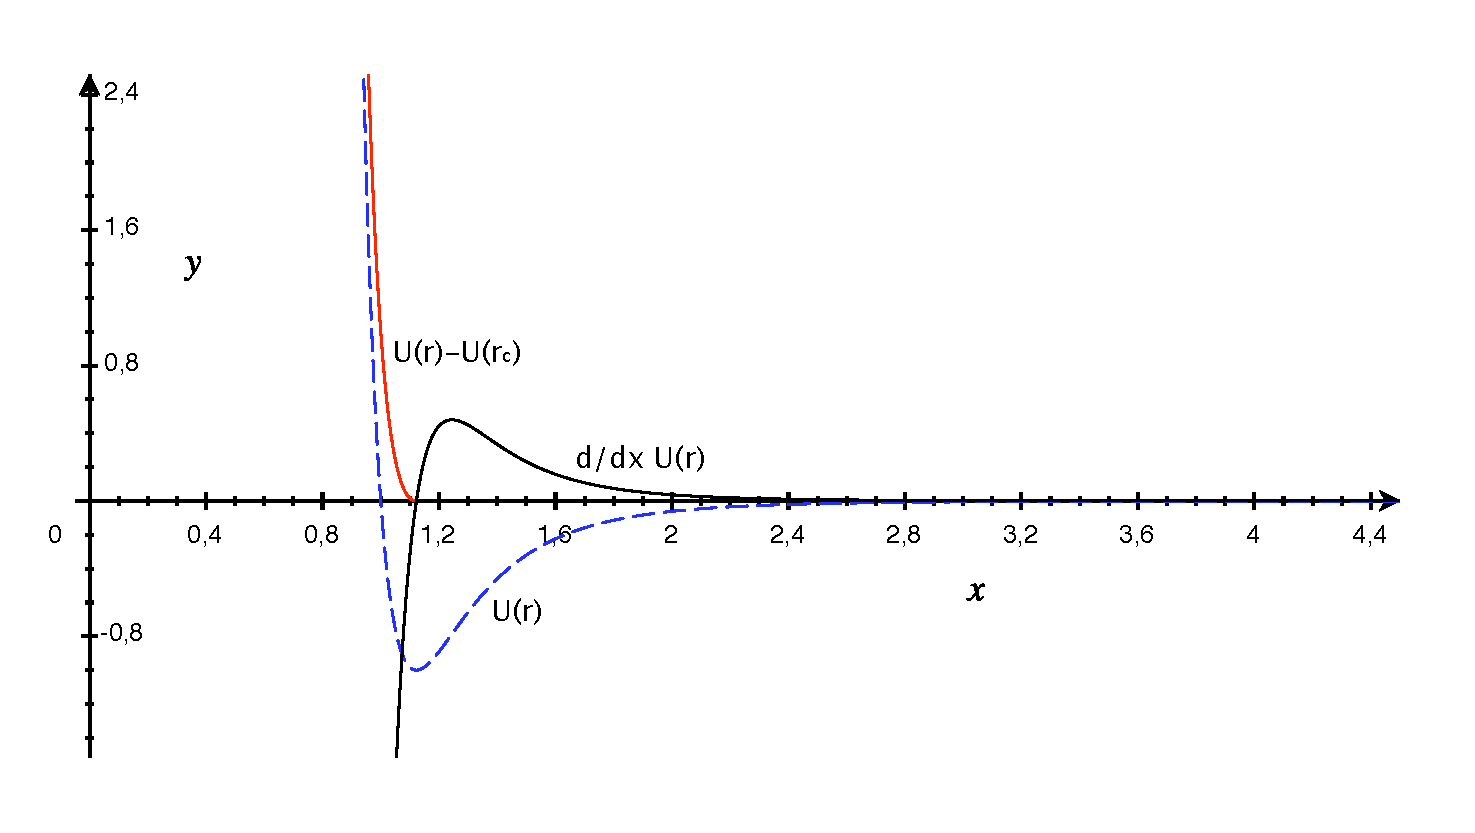
\includegraphics[width=0.75\textwidth]{figures/lennard-jones-potential.pdf}
\caption{\label{fig:lennard-jones} The Lennard Jones potentials as a function of the radial distance $r$ for two choices of the cut-off distance, the offset and shift; the interaction energy $\epsilon=1$ and radius of $\sigma=1$ are kept fixed. For a large cutoff such as $2.5\sigma$ the potential is practically zero at the cutoff (blue curve). The black curve shows the derivative of the L-J potential given by the blue curve. The red curve indicates the Weeks-Chandler-Andersen potential, which is obtained from the Lennard-Jones potential by cutting it off in its minimum at $r_c=\sqrt[6]{2}$ and shifting it up.}
\end{center}
\end{figure}

\subsection{Warming the system}
 
Now that we have set the necessary environment, we must `warm' our system before we can run the simulation. As we placed the particles at random positions in the box, some particles may overlap or be in very close proximity to each other. If this situation is allowed to exist \es{} will crash with the error: \texttt{particle out of range}. The enormous forces that the particles in close proximity experience during the initial time steps causes them to be propelled away from the center of the box at tremendous speed. To ensure that particles are sufficiently far apart to prevent such an `explosion' from happening, we set the Lennard-Jones force to a constant below a certain distance. Effectively, the divergent peak at $r = 0$ is cut off (capped) to some finite value.

To accomplish this capping, we use the \lstinline|inter forcecap| command. \textbf{N.B. The command in versions of \es{} predating the 3.1.1 release is \lstinline|inter ljforcecap| Please adjust your script according to the version you are using.} We perform the integration procedure  \verb"$warm_n_times" times for \verb"$warm_steps" steps and stop only if the minimal distance between particles is also larger than \verb"$min_dist", which was set earlier. To turn the capping off, we set \texttt{forcecap} to 0. 

{\small\vspace{0,2cm}
\begin{lstlisting}[firstnumber=auto]{bsp_code}
set cap 1.0
inter forcecap $cap

setmd time_step $tstep
set i 0
while { $i < $warm_n_times && $act_min_dist < $min_dist } 
{
    integrate $warm_steps

    set act_min_dist [analyze mindist]
    puts -nonewline "run $i at time = [setmd time] (LJ cap = $cap) min dist = $act_min_dist\r"
    flush stdout

    set cap [expr $cap+1.0]
    inter forcecap $cap
    incr i
}

inter forcecap 0
\end{lstlisting}\vspace{0,2cm}
}

\noindent In the above section of code you can see that the force capping is set to 1.0 initially. We subsequently set the integration time step and initialize the while loop. The loop ensures that warmup continues until the desired minimum separation between the particles is reached. Note that we implicitly assume that there is a sufficient number of integration steps; which for these parameters is true. An additional check with exit criterion can be built in, if necessary.

Inside the while loop, the system is integrated for \verb"$warm_steps", after which the minimum distance is analyzed and output. The command \texttt{-nonewline} ensures that \verb"puts" overwrites the command line, thereby showing the progress on a single line only. To prevent cashing the \texttt{stdout} stack must be flushed. Finally, the force cap is increased, to ensure that particles are pushed slowly but surely away from each other, and the interaction potential becomes more and more like the L-J potential. 

\subsection{Equilibration and production}

After we have set the necessary environment and warmed up our system, we can finally start with the actual simulation. We first equilibrate our system until all relevant physical observables are fluctuating around their mean values. In the case of Lennard Jones it is enough to monitor energy to see if the equilibration is successful. During equilibration, we (re)scale the particles' velocities to reach the target temperature, see the \texttt{lj\_functions.tcl} file for the scaling method used, in order to emulate the NVT ensemble by our $NVE$ simulation, as was explained earlier.

{\small\vspace{0,2cm}
\begin{lstlisting}[firstnumber=auto]{bsp_code}
setmd time_step $eq_tstep

for { set i 0 } { $i < $equilibration_iterations } { incr i } {
   integrate $equilibration_interval
   rescale_velocities $target_temperature $n_part
   puts -nonewline "equilibration run $i at time = [setmd time]\r"
   flush stdout
}
\end{lstlisting}\vspace{0,2cm}
}

\noindent The above code segment sets the time step for the integration to the right value. In the for loop, the system is integrated, the function \verb"rescale_velocities" is called to force the system towards the target temperature, and finally the result is output to the command line.

To analyze our data after the simulation, we need to open two files for writing the data to disk. 

{\small\vspace{0,2cm}
\begin{lstlisting}[firstnumber=auto]{bsp_code}
set blockfile [open "data/sim_info.dat" "w"]

set en [open "data/energy.dat" "w"]
puts $en "# Iteration Pressure Kinetic Potential Temperature Total"
\end{lstlisting}\vspace{0,2cm}
}

\noindent Note that the \verb"puts" command is used to put the header of the \texttt{data/energy.dat} into the \verb"en" stream. 

{\small\vspace{0,2cm}
\begin{lstlisting}[firstnumber=auto]{bsp_code}
setmd time_step $tstep

set nrep 0
for {set i 0} { $i < $sampling_iterations } { incr i} {
     incr nrep 

     integrate $sampling_interval

     save_sim $blockfile "id pos v f q type" "all"

     set energies [analyze energy]
     set pressure [analyze pressure total]
     set total [expr [lindex $energies 0 1]/$n_part]
     set kinetic [expr [lindex $energies 1 1]/$n_part]
     set potential [expr [lindex $energies 2 3]/$n_part]
     set temperature [expr $kinetic/1.5]
     puts $en "$i $pressure $kinetic $potential $temperature $total"

     lappend apressure $pressure
     lappend akinetic $kinetic
     lappend apotential $potential
     lappend atemperature $temperature
     lappend atotal $total

     puts -nonewline "integration step $i / $sampling_iterations\r"
     flush stdout
}

close $en
close $blockfile
\end{lstlisting}\vspace{0,2cm}
}

\noindent The above piece of code contains the production core of the simulation. We first reset the time step to the proper production value. We then set a counter to keep track of the number of cycles we that pass in the for loop. Inside this loop, we first increment the counter. We then integrate for the desired sampling length and save the state of the system using the  \lstinline|save_sim| statement. This statement calls the function defined in the \texttt{lj\_tutorial.tcl}. We tell the function what parameters are to be saved and for which particles we want to save these parameter (in this case `all'). N.B. We do not use velocity rescaling in the production part, since this would effectively eliminate the temperature fluctuations. 

Next we obtain the different system parameters from the simulation by calling the command \lstinline|analyze|. For instance the total, kinetic, and potential energy are obtained using the command \lstinline|analyze| \texttt{energy}. Note that we need to obtain the temperature from the kinetic energy of the system via the number of degrees of freedom, since we are still working in the microcanonical ensemble (N.B. we work with the energies per particle here). It should fluctuate around the preset temperature of the thermostat. Unfortunately, as mentioned, the $NVE$ ensemble does not yield the proper temperature fluctuations to model the $NVT$ ensemble.

We write the values for the iteration, the pressure, kinetic and potential energies, the temperature, and the total energy that we obtained to the \texttt{energy.dat} file using \lstinline|puts $en|. We also append the lists in which we store the system quantities during the production run, using the Tcl \lstinline|lappend| command. When the loop is finished, we close the \verb"en" and \verb"blockfile" streams, since we are done writing to disk.

\subsection{Simple error analysis on the time series data with \texttt{uwerr}}

As a last step before we finish our simulation, we calculate the mean values and statistical errors for the quantities we measured during the simulation. \es{} provides a build-in time series analysis tool called \lstinline|uwerr|. 

In our simulation we do not \emph{a priori} know if values of the same variable that we got from two adjacent samples are correlated or not. Sampling too seldom will lead either to long simulation runs or to bad statistics. On the other hand, sampling too often leads to strong correlations between the samples, which will make us underestimate the statistical errors in our measurements using usual formulas, e.g.~the standard deviation. \lstinline|uwerr| is used to determine the mean and the associated standard error, as well as the error on the error, of a quantity for an arbitrary numerical time series based on the article by Wolff~\cite{wolff}. Unlike the standard formulas, it can be used even with strongly correlated samples. See the code segment below for its implementation.

{\small\vspace{0,2cm}
\begin{lstlisting}[firstnumber=auto]{bsp_code}
puts "Reporting Energies and Temperature"

set error [uwerr $atotal $nrep 1 ]
set value [lindex $error 0]
set verror [lindex $error 1]
puts "  Total Energy: $value  $verror"

set error [uwerr $akinetic $nrep 1 ]
set value [lindex $error 0]
set verror [lindex $error 1]
puts "  Kinetic Energy: $value  $verror"

set error [uwerr $apotential $nrep 1 ]
set value [lindex $error 0]
set verror [lindex $error 1]
puts "  Potential Energy: $value  $verror"

set error [uwerr $atemperature $nrep 1 ]
set value [lindex $error 0]
set verror [lindex $error 1]
puts "  Temperature : $value  $verror"

set error [uwerr $apressure $nrep 1 ]
set value [lindex $error 0]
set verror [lindex $error 1]
puts "  Pressure : $value  $verror"
\end{lstlisting}\vspace{0,2cm}
}

\noindent To obtain, for example, the mean and error for the total energy, we submit as a first argument for \lstinline|uwerr| the array of all measured values of total energy \verb"$atotal", and then the total number of samples   \verb"$nrep". As the third argument we can give a `1', which means that we ran only one full measurement (complete simulation). \lstinline|uwerr| returns a string, the first value of which is the mean value for the physical quantity of interest and the second is the associated error.

\vspace{1cm}
\framebox{
\begin{minipage}{0.95\textwidth} 
\begin{task} \label{task:err}
Run the \texttt{lj\_tutorial.tcl} script for 5 different values of the initial seed, and compare the results of the \lstinline|uwerr| analysis of the temperature for the different runs. Note that there is a discrepancy between the statistical error on the mean value provided by \lstinline|uwerr| for each run and the spread in the mean values that you obtain for the different runs. Explain this. \newline

Hint: The thermostating during the equilibration run pushes the temperature towards the desired value, however the simulation enters the production run with a different total energy ($NVE$ ensemble) for every seed.
\end{task}
\end{minipage}}
\vspace{1cm}

In general, it is good practice to obtain the mean value from several simulations and \emph{obviously} in the correct ensemble. This requires us to provide \verb"$atotal" as a matrix, not as an array, to \lstinline|uwerr|. The total number of samples for every simulation should be the same and the third argument for \lstinline|uwerr| is then the number of simulations.

\vspace{1cm}
\framebox{
\begin{minipage}{0.95\textwidth} 
\begin{task}
Inspect what the \texttt{analyze pressure total} command returns. Make a similar error analysis for total pressure based on the information in the \texttt{energy.dat} file and compare this to the output given by the \lstinline|uwerr| command.\newline

Hint: \texttt{analyze pressure} (without \texttt{total}) returns the pressure and corresponding contributions to it.
\end{task}
\end{minipage}}
\vspace{1cm}

\noindent Finally, we need to exit \es{} using the following command

{\small\vspace{0,2cm}
\begin{lstlisting}[firstnumber=auto]{bsp_code}
exit
\end{lstlisting}\vspace{0,2cm}
}

\noindent Congratulations, you have now successfully executed your first Espresso simulation. 

\subsection{The \texttt{lj\_functions.tcl} file and the \lstinline|save_sim| function}

Before continuing with the analysis of the data that we obtained by our simulation, let us have a look at the \lstinline|save_sim| procedure in the \texttt{lj\_functions.tcl} file

{\small\vspace{0,2cm}
\begin{lstlisting}[numbers=none]
proc save_sim {cfile parinfo range} {
 blockfile $cfile write variable all
 blockfile $cfile write tclvariable all
 blockfile $cfile write particles $parinfo $range
 blockfile $cfile write interactions
 blockfile $cfile write bonds
 blockfile $cfile write random
 blockfile $cfile write seed
 blockfile $cfile write bitrandom
 blockfile $cfile write bitseed
}
\end{lstlisting}\vspace{0,2cm}
}

\noindent 
This procedure saves all variables available in our program to the \lstinline|$cfile| stream, which in our example is set to \texttt{sim\_info.dat}, which is located in the \texttt{data} directory. 

\vspace{1cm}
\framebox{
\begin{minipage}{0.95\textwidth} 
\begin{task}
Study the file \texttt{lj\_functions.tcl}, specifically the procedure \lstinline|save_sim| and how it is called in \texttt{lj\_tutorial.tcl} file. Then run \texttt{lj\_tutorial.tcl} and check the \texttt{data} directory for the simulation data file \texttt{sim\_info.dat} and inspect it. 
\end{task}
\end{minipage}}
\vspace{1cm}

\noindent Below we give a sample of the output produced by the \lstinline|save_sim| procedure:

{\small\vspace{0,2cm}
\begin{verbatim}
{variable 
	{box_l 5.2387886 5.2387886 5.2387886}
	{cell_grid 2 2 2}
	{cell_size 2.6193943 2.6193943 2.6193943}
	{dpd_gamma 0.0}
	{dpd_r_cut 0.0}
	...
}
{tclvariable 
	{density 0.8442}
	{tstep 0.001}
	{lj1_cut 2.5}
	{blockfile file12}
	...
}
{particles {id pos v f q type} 
	{0 13.08106 4.376436 2.4466876 1.2432192 ...}
	{1 -2.7657422 -0.09919841 -1.0362237 -0.4642931...}
	{2 4.4635587 5.4885591 5.460385 0.18670765 ...}
	{3 -2.9920063 0.88519503 7.3518191 0.5820964 ...}
	...
}
{interactions 
	{0 0 lennard-jones 1.0 1.0 2.5 0.0040792228 0.0 0.0 }
}
{bonds  
	{0 { } }
	{1 { } }
	...
}
{random 
	{1198928294 .... }
}
{seed 
	{16838}
}
{bitrandom 
	{0 147 2085679233 .... }
}	
{bitseed 
	{16838}
}
...
\end{verbatim}
\vspace{0,2cm}
}

\noindent You will find there are nine types of blocks which are repeated very often. The first block (\texttt{variable}) contains all \es{} variables, the second (\texttt{tclvariable}) all variables of the tcl script. In the third block we find the particle data that we told the \lstinline|save_sim| function to save (id: particle id, pos: position, v: velocity, f: force, q: charge, type). The function \lstinline|save_sim| also saves interactions, bonds, random numbers used, the seed for the random number generator, and (equivalently) the bitrandom and bitseed numbers. 

In our case the interaction is given by the Lennard-Jones potential. The bonds block is empty because the particles are not bound to each other, like in, for example, a polymer. The rest of the blocks contain information (random, seed, bitrandom and bitseed) that is required to restore the random generator after quiting \es{}. This may be useful when you partition a run into several pieces, terminating \es{} after each part. Using the last blocks it is possible to start subsequent runs, in such a way that the result is \emph{exactly} the same, as if you had run a single long run with the same seed.

Looking at the \texttt{lj\_tutorial.tcl} script, we see that the \lstinline|save_sim| function is called every time in the loop; that is why the blocks are repeated. N.B. Writing away the full state of the system this often does eat up a sizable chunk of drive space, for the parameters set in our simulation around 2.7 GB.

\section{\label{sec:ana}Analyzing the Data Obtained from the \es{} L-J Fluid Simulation}

In this section we will show several ways of analyzing the data generated by our \es{} simulation. 

\subsection{Checking the equilibration of the data}

\begin{figure}[!ht]
\begin{center}
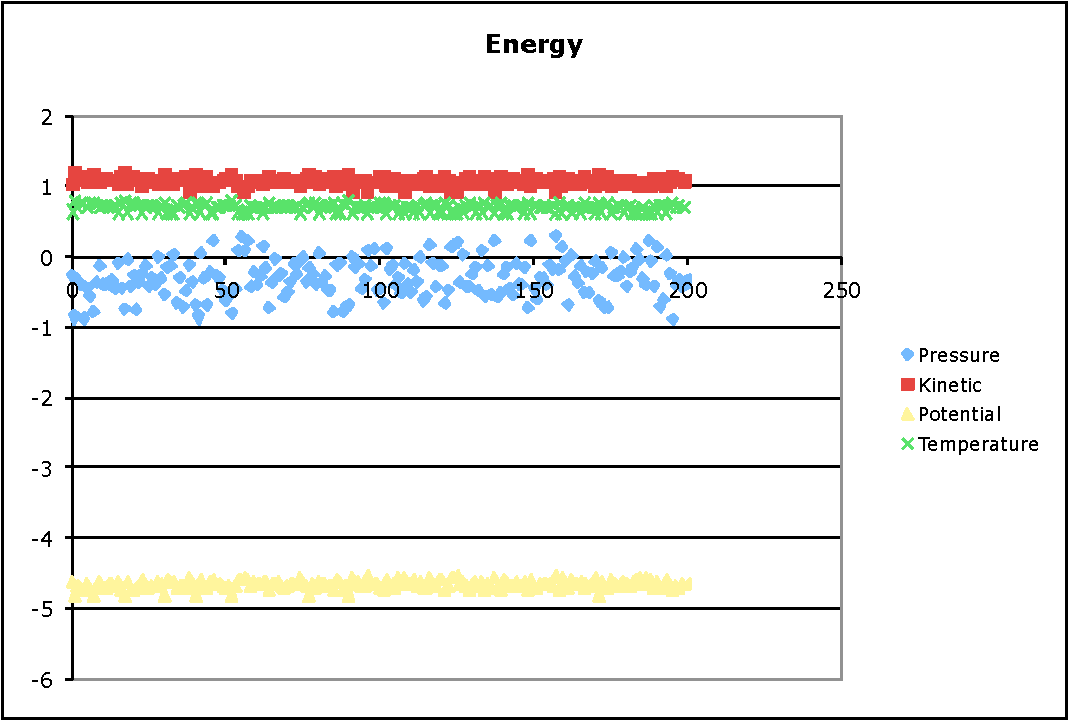
\includegraphics[width=\textwidth]{figures/energy}
\caption{\label{fig:energy} The physical quantities extracted from the simulation as a function of the number of production cycles $N$. We show the results in reduced units. Note that, as is to be expected for the $NVE$ ensemble, the total energy is constant. Also note that the fluctuations around the averages are significant, since we only have 108 particles.}
\end{center}
\end{figure}

\vspace{1cm}
\framebox{
\begin{minipage}{0.95\textwidth} 
\begin{task}
Plot the time evolution of the pressure and energy, which are written into the \texttt{data} directory in the file \texttt{energy.dat}.\newline

Hint: you can modify the \texttt{gnuplot} script \texttt{script\_energy} that is provided with the tutorial to generate the desired graph.
\end{task}
\end{minipage}}
\vspace{1cm}

\noindent The quantities in the \texttt{energy.dat} file are shown as a function of the number of production run cycles in Fig.~\ref{fig:energy}. As we can see the system is in equilibrium because pressure, potential and kinetic energy per particle, and the current temperature fluctuate around their mean values.

\subsection{Average velocity of the particles}

In this and the following sections, we will work with the other Tcl scripts that were provided in the tutorial folder. 

\vspace{1cm}
\framebox{
\begin{minipage}{0.95\textwidth} 
\begin{task} \label{task:avvel}
Study and run the script \texttt{blockfile\_read.tcl}. The script reads in data from the \texttt{data/sim\_info.dat} file which was generated by the \lstinline|save_sim| function from the \texttt{lj\_functions.tcl} script.\newline

Modify this script to determine the average particle velocity, i.e. $\langle \vert \mathbf{v} \vert^{2} \rangle$ of the first particle in the `naive' way and compare this to what you expect based on the average temperature of the system.
\end{task}
\end{minipage}}
\vspace{1cm}

We first consider the \texttt{blockfile\_read.tcl} script. In its current state it sets a file name and uses the \lstinline|open| command with the ``r'' key to open a read stream to the \texttt{data/sim\_info.dat} file. It then proceeds to read in the data block by block until it has reached the end of the file using the \lstinline|blockfile| command, see below.

{\small\vspace{0,2cm}
\begin{lstlisting}[numbers=none]
set filename "data/sim_info.dat"
set in [open "$filename" "r"]

while {  [set btitle [ blockfile $in read auto ] ] != "eof" } {

  if {$btitle == "variable"} {
    set times [setmd time]
  }

  if { $btitle == "particles"} {
    set part0 [part 0 print pos]
    set part0v [part 0 print v]
    puts "time = $times"
    puts "position of the first particle = $part0"
    puts "velocity of the first particle = $part0v\n"
  }
}

close $in
exit
\end{lstlisting}\vspace{0,2cm}
}

\noindent The \lstinline|blockfile| statement requires the data stream, in this case \texttt{\$in}, and is given the task to read \texttt{auto}, which implies that it reads all blocks regardless of their title, e.g. ``particles'' or ``bitrandom''.

The blocks that are read in are then analyzed. From the ``variable'' blocks the simulation time is extracted and from the ``particle'' blocks the velocities are extracted. The reason for the if statement is on the one hand to prevent to time and velocities being reset for every one of the 9 blocks that constitute a snapshot. On the other, certain data is only available after a specific block has been read in. The quantities we read are subsequently output to the command line. Finally, the stream is closed and the script exits \es{}.

\textbf{Possible solution to Task~\ref{task:avvel}:} Using the Tcl interface we can now modify the script to determine the average squared velocity $\langle \vert v(t) \vert^{2} \rangle$ of one of our particles. To do this we require three additional variables

{\small\vspace{0,2cm}
\begin{lstlisting}[numbers=none]
set filename "data/sim_info.dat"
set in [open "$filename" "r"]

set vel2 0.0
set count 0

while { [set btitle [ blockfile $in read auto ] ] != "eof" } {
  if { $btitle == "particles"} {
    incr count;
    set part0v [part 0 print v]
    set vel2 [expr $vel2 + ([lindex $part0v 0]*[lindex $part0v 0] \
      + [lindex $part0v 1]*[lindex $part0v 1] \
      + [lindex $part0v 2]*[lindex $part0v 2])]
    set av_vel2 [expr $vel2/$count]

    puts -nonewline "the instantaneous average squared velocity of the first particle = $av_vel2 \r"
    flush stdout
  }
}

puts "\n the average squared velocity of the first particle = $av_vel2"

close $in
exit
\end{lstlisting}\vspace{0,2cm}
}

\noindent Note that we need to increment the counter in the \lstinline|if| statement, since there are several blocks which do not have the ``particles'' label, which are also read in. We obtain $\langle \vert \mathbf{v} \vert^{2} \rangle \approx 2.1$. We also know by applying the equipartition theorem to our system that $\langle \vert \mathbf{v} \vert^{2} \rangle = 3 T$, from this we find that $T \approx 0.7$ (the results are too inaccurate to give more decimal precision). Remember from the L-J simulation we obtained an average temperature of $\langle T \rangle = 0.714 \pm 0.02$ (see Task~\ref{task:err}) and that the \lstinline|uwerr| average is $\langle T \rangle \approx 0.68$. We therefore find good correspondence between the two results. Remember we only consider one particle and one run here, if we take an average over all particles and multiple runs, the correspondence will be better. Of course, the method by which the average temperature was calculated in the \texttt{lj\_tutorial.tcl} was essentially the same.

\subsection{The radial distribution function}

\begin{figure}[!ht]
\begin{center}
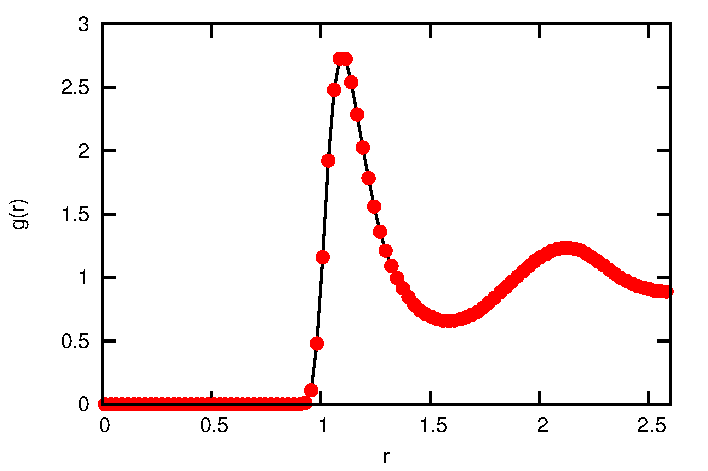
\includegraphics[width=0.75\textwidth]{figures/rdf}
\caption{\label{fig:rdf} The radial distribution function $g(r)$ for a L-J particle in the fluid environment that we simulated.}
\end{center}
\end{figure}

The radial distribution function (RDF) describes the distribution of particles around the center of a fixed particle, as a function of the particle-particle distance. This of course assumes that the particle distribution is isotropic around the particles. The radial distribution function is of fundamental importance in thermodynamics because it can be used to obtain macroscopic thermodynamic quantities, such as the pressure in the system. We do not go into this here, however, since these calculations are nontrivial.

\vspace{1cm}
\framebox{
\begin{minipage}{0.95\textwidth} 
\begin{task}  
Run the \texttt{rdf.tcl} script, inspect the code and see what each component does. Plot the RDF from the file \texttt{data/rdf.dat} that is generated by the script. Try different parameters for the \texttt{analyze rdf} command, such as the bin size. What do you observe?\newline

Hint: You can use the \texttt{gnuplot} script \texttt{script\_rdf} to plot the RDF. 
\end{task}
\end{minipage}}
\vspace{1cm}

\noindent Note that we obtain a RDF which shows liquid properties. That is to say, a peak near one particle diameter and another, broader peak near twice the particle diameter. This result is typical for a fluid, where one can think of a central fluid particle, surrounded by spherical shells of neighboring particles. It is strongly dissimilar from a crystal RDF, where the periodicity of the lattice induces sharp peaks at distances related to the morphology of the crystal. Determining the correct bin size for the RDF can be tricky, since with increased bin size, the number of points in the graph will be greater, but the curve will be less smooth due to poorer sampling. 

\subsection{The velocity auto-correlation function}

The velocity auto-correlation function (VACF) is an averaged time-dependent correlation function of all particles' velocities. It can be used to elucidate the dynamical processes that underlie the behavior of the system. That is, it gives information on the likelihood that two observations separated by a given time will yield similar results. Moreover, the VACF may be integrated to determine the self-diffusion coefficient $D$. Let us first begin by calculating the VACF for our L-J liquid system.  

\vspace{1cm}
\framebox{
\begin{minipage}{0.95\textwidth} 
\begin{task} \label{task:vacf}
Run the \texttt{vacf.tcl} script and see if you can follow the code. Plot the VACF from \texttt{data/vacf.dat} using the \texttt{gnuplot} script \texttt{script\_vacf}. The VACF correlation $C(t)$ can be computed directly as: \[ C(t) = \langle {\bf v}_{i} (0) \cdot {\bf v}_{i}(t) \rangle \] This exact result can be approximated by \[ C(t) = \frac {1} {N} \sum_{i=0}^{N} {\bf v}_{i} (0) \cdot {\bf v}_{i} (t) \] where $N$ is the number of particles. Note that this VACF is not normalized to unity when the data is fully correlated. Try to modify \texttt{vacf.tcl} by using tcl vector and math functions, see the User Guide for more information.
\end{task}
\end{minipage}}
\vspace{1cm}

\begin{figure}[!ht]
\begin{center}
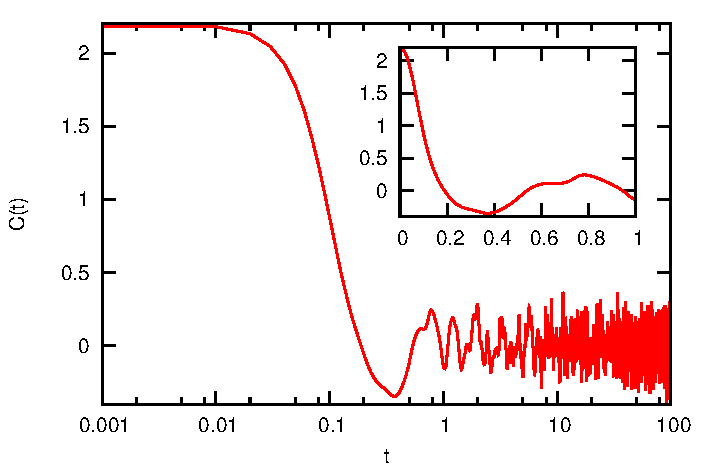
\includegraphics[width=0.75\textwidth]{figures/vacf}
\caption{\label{fig:vacf} The velocity auto-correlation function $C(t)$ for a L-J particle in the fluid environment that we simulated. The main graph shows a log-linear plot, and the inset shows a regular plot of the domain $t \in [0,1]$. Note the significant noise for the long-time $C(t)$ values.}
\end{center}
\end{figure}

\noindent The VACF in Fig.~\ref{fig:vacf} shows the following. Initially, for $t \ll 1$ $C(t)$ has negligible slope. This is caused by the fact that on short time scales (for soft-interactions) the particles have not interacted strongly with each other. That is, the particles' initial velocity is virtually unaffected by the presence of other particles. Note that this would not be the case for a hard sphere fluid, where the decay of $C(t)$ sets in immediately. In the L-J fluid, the particles move towards locations, where there is a balance between the repulsive and attractive forces that they experience. These positions are energetically stable. One would therefore expect the motion of the particle to be an oscillatory one around such a minimum. However, in the liquid the particles also diffuse. This diffusion quickly eliminates the oscillatory motion.

It is therefore (typically) possible to find only one overdamped oscillation in the fluid, which can be thought of as a collision between two particles, leading to a rebound (back-scattering event), before they diffuse away. This rebound leads to the first minimum in $C(t)$, which assumes negative values, since the particles will in general move in the opposite direction after a collision event. Diffusion typically causes the VACF to decay asymptotically to zero after a possible (small) local maximum following the rebound minimum. However, this cannot be appreciated from Fig.~\ref{fig:vacf}, due to the poor averaging at time scales $t > 0.2$.  

\textbf{Possible solution to Task~\ref{task:vacf}:} The following script gives exactly the same result (barring small numerical deviations in the last decimals), as the original script \texttt{vacf.tcl}. However, we have significantly reduced the length of the script, by making use of the Tcl vector and list operators.

{\small\vspace{0,2cm}
\begin{lstlisting}[numbers=none]
set filename "data/sim_info.dat"
set in [open "$filename" "r"]
set out [open "data/vacf.dat" "w"]

set origin 0
while {  [set btitle [ blockfile $in read auto ] ] != "eof" } {

  if { $btitle == "particles"} {

    if {$origin == 0} {
      set time0 [setmd time]
    }
    set times [setmd time]
    set pmax [setmd n_part]

    if {$origin == 0} {
      for {set i 0} {$i < $pmax} {incr i} {
        lappend vec0 [part $i print v]
      }
      set origin 1
    }

    set acf 0.0
    for {set i 0} {$i < [llength $vec0]} {incr i} {
      set v1 [part $i print v]
      set v0 [lindex $vec0 $i]
      set acf [expr $acf + [vecdot_product $v1 $v0]]
    }
    set acf [expr $acf/$pmax]

    puts $out "[expr $times - $time0] $acf"
  }
}

close $in
close $out
exit
\end{lstlisting}\vspace{0,2cm}
}

\noindent It is also possible to calculate the VACF in \es{} during the simulation (version 3.1.1 onward), instead of determining it using post processing. This method makes use of the (new) \lstinline|observables| and \lstinline|correlation| functions that are implemented in \es{} 3.1.1 onward. We refer to the User Guide for more information on these functions. In the tutorial \texttt{lj\_tutorial\_vacf.tcl} we have implemented these functions to determine $C(t)$. The essential modifications can be summarized in the following piece of code:

{\small\vspace{0,2cm}
\begin{lstlisting}[numbers=none]
setmd time_step $tstep
set tmax 10.0
set delt [expr $tstep*$sampling_interval]

set vel_id [observable new particle_velocities type 0]

set vacf [correlation new obs $vel_id corr_operation scalar_product dt $delt tau_max $tmax]

for {set i 0} { $i < $sampling_iterations } { incr i } {
     integrate $sampling_interval
     correlation $vacf update
}

correlation $vacf finalize
correlation $vacf write_to_file "data/vacf_internal.dat"
\end{lstlisting}\vspace{0,2cm}
}

\noindent In the first line we set the time step for the production run as before. We then define the maximum time interval we are interested in. Note that if the time interval is set too large, there is a substantial computational overhead to the correlation function, which slows down \es{} significantly. We also set the time step for the correlation. N.B. In our case this has to be the time step times the integration interval size. Next we set the observable we are interested in. In this case the particle velocities of particles with type 0. Finally, we define the correlation that we want to determine. We pass the observable \texttt{\$vel\_id} and the type of mathematical operation we want to perform to obtain the correlation; in this case as scalar (inner) product \texttt{scalar\_product}. We also specify the time step using \texttt{dt \$delt} and the maximum correlation time of interest \texttt{tau\_max}.

\begin{figure}[!ht]
\begin{center}
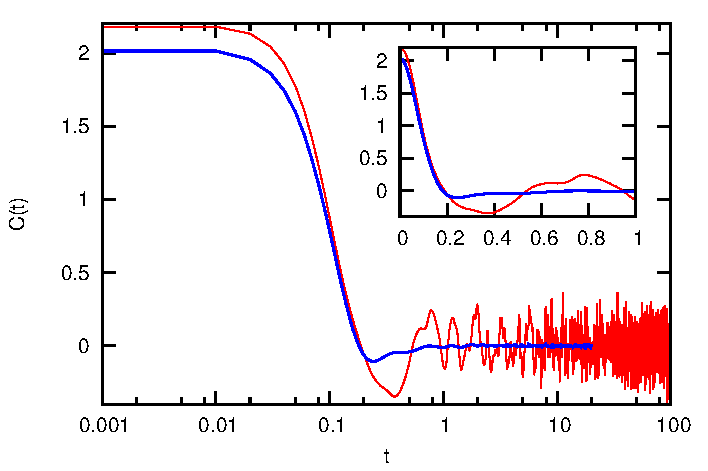
\includegraphics[width=0.75\textwidth]{figures/vacf_internal}
\caption{\label{fig:vacf_internal} Comparison between the velocity auto-correlation function $C(t)$ for a L-J particle in the fluid environment as calculated by the internal \es{} \lstinline|correlation| function (blue thick) and the results of our script \texttt{vacf.tcl} (red thin). The main graph shows a log-linear plot, and the inset shows a regular plot of the domain $t \in [0,1]$. Note the significant decrease in numerical noise achieved by the much more advanced \es{} routine. The short time features are qualitatively the same, but deviations start to set in at intermediate times. From the improved data set the long-time (asymptotic) decay can be more readily appreciated. For $t \gg 1$ we again encounter numerical noise, but it is significantly reduced.}
\end{center}
\end{figure}

\noindent After setting up the correlation function, we start the integration. During the integration we update the velocity auto-correlation function. After the production run we finalize the result, i.e., make sure that the correlation is fully updated. Currently, \es{} returns \texttt{tau\_lin: 1000} as output, which simply means that there were 1000 linear time steps in the correlation interval. Finally, we write the result of the computation to the file \texttt{data/vacf\_internal.dat}. This file consists of three columns. The first gives the time, the second gives the number of samples for each interval and the third the value of the correlation. Note that this correlation is not expressed in `per particle' terms. The \texttt{gnuplot} script \texttt{script\_vacf\_internal} therefore compensates for this, see Fig.~\ref{fig:vacf_internal} for the result of \es{}'s internal correlation routine. 

\noindent Unfortunately, even the VACF calculated using \es{}'s internal routines is of insufficient quality to calculate the diffusion coefficient. In general the procedure to determine the diffusion coefficient $D$ would be to numerically determine the following integral
\begin{equation}
\label{eq:diff} D  = \frac{1}{3} \int_{0}^{\infty} \mathrm{d}t C(t) 
\end{equation}
However, this requires high quality VACF data. Another way to extract the diffusion coefficient is by determining the mean-square displacement.

\subsection{The mean-square displacement}

\vspace{1cm}
\framebox{
\begin{minipage}{0.95\textwidth} 
\begin{task} \label{task:msd}
Run \texttt{msd.tcl} and try to understand the code. Use the \texttt{gnuplot} script \texttt{script\_msd} to plot the MSD from the file \texttt{data/msd.dat}. The MSD can be simply computed by: \[ \langle \Delta r^{2}(t) \rangle  = \frac {1} {N} \sum_{i=0}^{N} \Delta {\bf r}_{i}^{2} (t)\] or \[ \langle \Delta r^{2} (t)  \rangle = \frac {1} {N} \sum_{i=0}^{N} | r_{i}(t)-r_{i}(0) | ^{2} \] \newline
Note that the MSD is a type of correlation function. Read through the User Guide and figure out how to implement the MSD in the \es{} tutorial file \texttt{lj\_tutorial.tcl} in a similar fashion as you did for the VACF.
\end{task}
\end{minipage}}
\vspace{1cm}

The mean-square displacement (MSD) is the average squared distance that a particle traveled during a given time. The MSD contains information on the diffusion of particles. See Fig.~\ref{fig:msd} for the mean-square displacement of the particles in our system. 

\begin{figure}[!ht]
\begin{center}
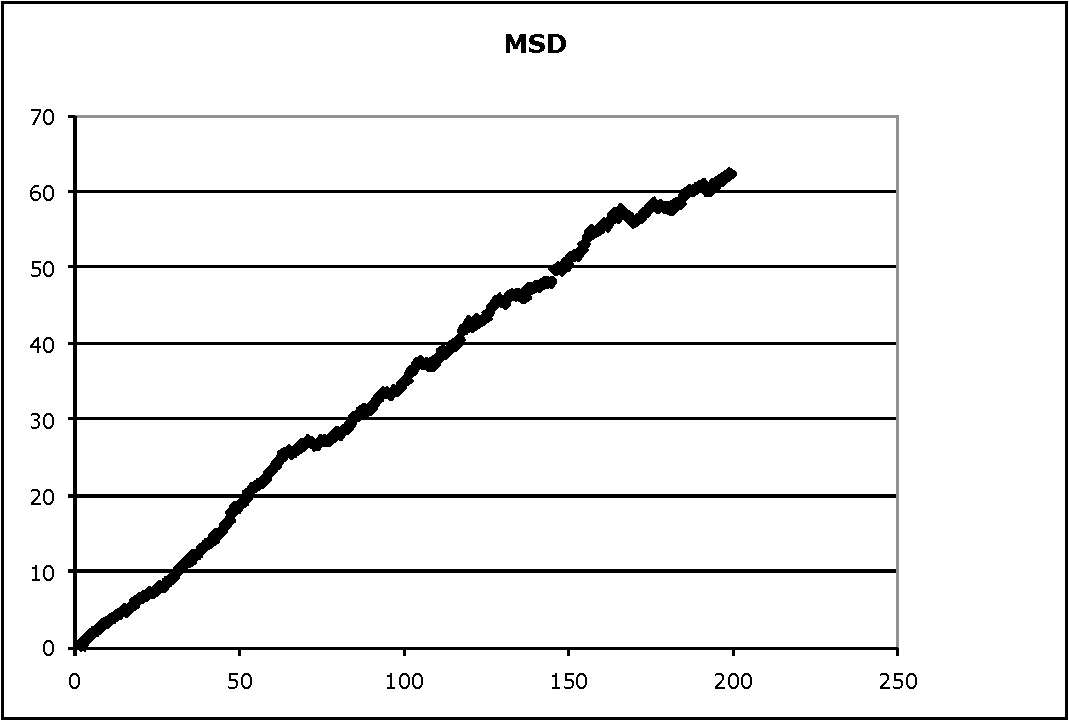
\includegraphics[width=0.75\textwidth]{figures/msd}
\caption{\label{fig:msd} The mean-square displacement $\langle \Delta r^{2}(t)  \rangle$ for a L-J particle in the fluid environment that we simulated. The main graph shows a linear plot, and the inset shows a log-log plot, in which the ballistic and diffusive regimes can be more easily differentiated. The green line indicates that $\langle \Delta r^{2}(t)  \rangle \propto t^2$ in the ballistic regime and the blue line that $\langle \Delta r^{2}(t) \rangle \propto t$ in the diffusive regime.}
\end{center}
\end{figure}

On short time scales the particles do not collide/interact with the other particles (ballistic regime). This is essentially the regime for which the VACF remains constant. In this regime, the distance traveled is be proportional to the time and therefore the MSD should increase quadratically. For larger time scales, the particle interacts with the other particles. This causes the particle to perform a random walk, each collision giving it a new direction of motion. This regime is called the diffusive regime, and is characterized by a linear increase of the MSD with time. The coefficient of proportionality is the diffusion coefficient: $D = \langle \Delta r^2(t) \rangle/(2 d t)$, where $d$ is the dimensionality of the problem and $t$ the traveling time. A simple linear fit to the data in the interval $t \in [1,100]$ gives us the value $D = (4.8 \pm 0.3) \cdot 10^{-2}$. Again, the mean and standard deviation are only valid for this single production run, to obtain a more accurate mean and standard deviation we should average over multiple production runs.

\textbf{Possible solution to Task~\ref{task:msd}:} The essential modifications can be summarized in the following piece of code

{\small\vspace{0,2cm}
\begin{lstlisting}[numbers=none]
setmd time_step $tstep
set tmax 25.0

set delt [expr $tstep*$sampling_interval]

set pos_id [observable new particle_positions type 0]

set msd [correlation new obs $pos_id corr_operation square_distance_componentwise dt $delt tau_max $tmax]

for {set i 0} { $i < $sampling_iterations } { incr i } {
     integrate $sampling_interval
     correlation $msd update
}

correlation $msd finalize
correlation $msd write_to_file "data/msd_internal.dat"
\end{lstlisting}\vspace{0,2cm}
}

Note that the output file \texttt{data/msd\_internal.dat} is quite different from the one we obtained for the VACF. For each particle and for each coordinate ($x$, $y$ and $z$) the MSD has been determined separately. To compare with the MSD that we obtained by our Tcl script, we need to average over all particles and coordinates. This is allowed since in the fluid all directions are equivalent. If we do so, we obtain the following result, see Fig.~\ref{fig:msd_internal} for a comparison to the MSD generated by the \texttt{msd.tcl} script. Note that we were able to determine statistical errors here for each $t$, since we could compare the MSD data of the different particles.

\begin{figure}[!ht]
\begin{center}
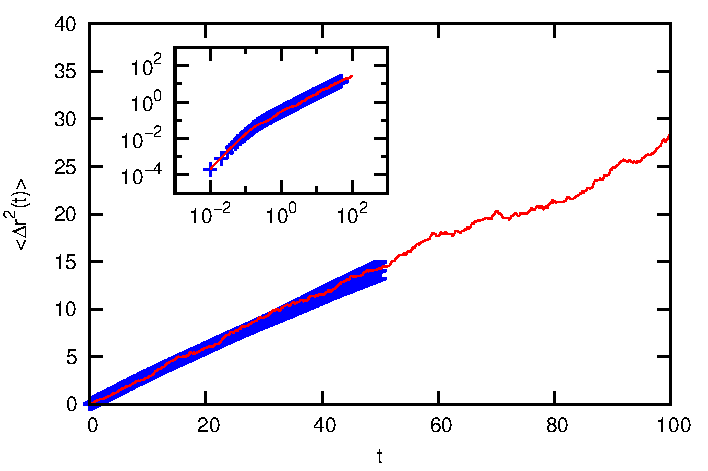
\includegraphics[width=0.75\textwidth]{figures/msd_internal}
\caption{\label{fig:msd_internal} Comparison between the mean-square displacement $\langle \Delta r^2(t) \rangle$ for a L-J particle in the fluid environment as calculated by the internal \es{} \lstinline|correlation| function (blue thick; with error bars) and the results of our script \texttt{msd.tcl} (red thin).The main graph shows a linear plot, and the inset shows a log-log plot, in which the ballistic and diffusive regimes can be more easily differentiated. Note the significant decrease in numerical noise achieved by the much more advanced \es{} routine.}
\end{center}
\end{figure}

Using the \es{} MSD calculation, we can now again determine the diffusion coefficient $D = (4.9 \pm 0.1)\cdot10^{-2}$. Note that the values for $D$ are in agreement for this single run. 

\vspace{1cm}
\framebox{
\begin{minipage}{0.95\textwidth} 
\begin{task}
Now that you have a good understanding of the Tcl language, the \es{} command structure and the ways to analyze data, you should try to set up a L-J fluid simulation that uses the proper $NVT$ ensemble. Compare the average values for the quantities of interest, as well as the MSD and VACF you obtain.\newline

Hint: Use the Langevin thermostat. 
\end{task}
\end{minipage}}
\vspace{1cm}

\bibliographystyle{unsrt}
\bibliography{refs}

\end{document}

